\section{Sudoku}

Sudoku puzzle is a 9*9 grid with some cells filled with values, some are empty:

% copypasted from http://www.texample.net/tikz/examples/sudoku/
\newcounter{row}
\newcounter{col}

\newcommand\setrow[9]{
  \setcounter{col}{1}
  \foreach \n in {#1, #2, #3, #4, #5, #6, #7, #8, #9} {
    \edef\x{\value{col} - 0.5}
    \edef\y{9.5 - \value{row}}
    \node[anchor=center] at (\x, \y) {\n};
    \stepcounter{col}
  }
  \stepcounter{row}
}

\begin{center}
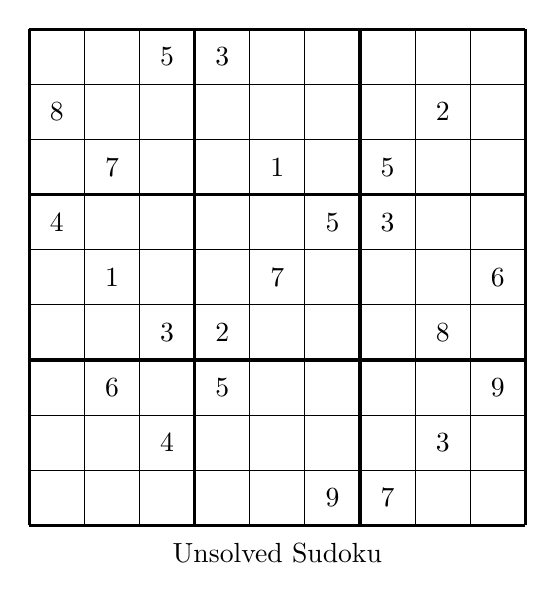
\begin{tikzpicture}[scale=.7]
  \begin{scope}
    \draw (0, 0) grid (9, 9);
    \draw[very thick, scale=3] (0, 0) grid (3, 3);

    \setcounter{row}{1}
    \setrow { }{ }{5}  {3}{ }{ }  { }{ }{ }
    \setrow {8}{ }{ }  { }{ }{ }  { }{2}{ }
    \setrow { }{7}{ }  { }{1}{ }  {5}{ }{ }

    \setrow {4}{ }{ }  { }{ }{5}  {3}{ }{ }
    \setrow { }{1}{ }  { }{7}{ }  { }{ }{6}
    \setrow { }{ }{3}  {2}{ }{ }  { }{8}{ }

    \setrow { }{6}{ }  {5}{ }{ }  { }{ }{9}
    \setrow { }{ }{4}  { }{ }{ }  { }{3}{ }
    \setrow { }{ }{ }  { }{ }{9}  {7}{ }{ }

    \node[anchor=center] at (4.5, -0.5) {Unsolved Sudoku};
  \end{scope}
\end{tikzpicture}
\end{center}

Numbers of each row must be unique, i.e., it must contain all 9 numbers in range of 1..9 without repetition.
Same story for each column and also for each 3*3 square.

This puzzle is good candidate to try \ac{SMT} solver on, because it's essentially an unsolved system of equations.

\subsubsection{Simple sudoku in SMT}
\label{sudoku_SMT}

\paragraph{The first idea}

The only thing we must decide is that how to determine in one expression, if the input 9 variables has all 9 unique numbers?
They are not ordered or sorted, after all.

From the school-level arithmetics, we can devise this idea:

\begin{equation}
\underbrace{10^{i_1} + 10^{i_2} + \cdots + 10^{i_9}}_9 = 1111111110
\end{equation}

Take each input variable, calculate $10^i$ and sum them all.
If all input values are unique, each will be settled at its own place.
Even more than that: there will be no holes, i.e., no skipped values.
So, in case of Sudoku, 1111111110 number will be final result, indicating that all 9 input values are unique, in range of 1..9.

Exponentiation is heavy operation, can we use binary operations? Yes, just replace 10 with 2:

\begin{equation}
\underbrace{2^{i_1} + 2^{i_2} + \cdots + 2^{i_9}}_9 = 1111111110_2
\end{equation}

The effect is just the same, but the final value is in base 2 instead of 10.

Now a working example:

\lstinputlisting[style=custompy]{puzzles/sudoku/1/sudoku_plus_Z3.py}
( \url{https://github.com/DennisYurichev/SAT_SMT_by_example/blob/master/puzzles/sudoku/1/sudoku_plus_Z3.py} )

\begin{lstlisting}
% time python sudoku_plus_Z3.py
1 4 5 3 2 7 6 9 8
8 3 9 6 5 4 1 2 7
6 7 2 9 1 8 5 4 3
4 9 6 1 8 5 3 7 2
2 1 8 4 7 3 9 5 6
7 5 3 2 9 6 4 8 1
3 6 7 5 4 2 8 1 9
9 8 4 7 6 1 2 3 5
5 2 1 8 3 9 7 6 4

real    0m11.717s
user    0m10.896s
sys     0m0.068s
\end{lstlisting}

Even more, we can replace summing operation to logical OR:

\begin{equation}
\underbrace{2^{i_1} \vee 2^{i_2} \vee \cdots \vee 2^{i_9}}_9 = 1111111110_2
\end{equation}

% FIXME: только часть исходника
\lstinputlisting[style=custompy]{puzzles/sudoku/1/sudoku_or_Z3.py}
( \url{https://github.com/DennisYurichev/SAT_SMT_by_example/blob/master/puzzles/sudoku/1/sudoku_or_Z3.py} )

Now it works much faster. Z3 handles OR operation over bit vectors better than addition?

\begin{lstlisting}
% time python sudoku_or_Z3.py
1 4 5 3 2 7 6 9 8
8 3 9 6 5 4 1 2 7
6 7 2 9 1 8 5 4 3
4 9 6 1 8 5 3 7 2
2 1 8 4 7 3 9 5 6
7 5 3 2 9 6 4 8 1
3 6 7 5 4 2 8 1 9
9 8 4 7 6 1 2 3 5
5 2 1 8 3 9 7 6 4

real    0m1.429s
user    0m1.393s
sys     0m0.036s
\end{lstlisting}

The puzzle I used as example is dubbed as one of the hardest known
\footnote{\url{http://www.mirror.co.uk/news/weird-news/worlds-hardest-sudoku-can-you-242294}} (well, for humans).
It took $\approx 1.4$ seconds on my Intel Core i3-3110M 2.4GHz notebook to solve it.

\paragraph{The second idea}

My first approach is far from effective, I did what first came to my mind and worked.
Another approach is to use \TT{distinct} command from SMT-LIB, which tells Z3 that some variables must be distinct (or unique).
This command is also available in Z3 Python interface.

I've rewritten my first Sudoku solver, now it operates over \textit{Int} \textit{sort}, it has \TT{distinct} commands instead of bit operations,
and now also other constaint added: each cell value must be in 1..9 range, because, otherwise, Z3 will offer (although correct) solution with too big
and/or negative numbers.

% FIXME: только часть исходника
\lstinputlisting[style=custompy]{puzzles/sudoku/1/sudoku2_Z3.py}
( \url{https://github.com/DennisYurichev/SAT_SMT_by_example/blob/master/puzzles/sudoku/1/sudoku2_Z3.py} )

\begin{lstlisting}
% time python sudoku2_Z3.py
1 4 5 3 2 7 6 9 8
8 3 9 6 5 4 1 2 7
6 7 2 9 1 8 5 4 3
4 9 6 1 8 5 3 7 2
2 1 8 4 7 3 9 5 6
7 5 3 2 9 6 4 8 1
3 6 7 5 4 2 8 1 9
9 8 4 7 6 1 2 3 5
5 2 1 8 3 9 7 6 4

real    0m0.382s
user    0m0.346s
sys     0m0.036s
\end{lstlisting}

That's much faster.

\paragraph{Conclusion}

\ac{SMT}-solvers are so helpful, is that our Sudoku solver has nothing else, we have just defined relationships between variables (cells).

\paragraph{Homework}

As it seems, true Sudoku puzzle is the one which has only one solution.
The piece of code I've included here shows only the first one.
Using the method described earlier (\ref{SMTEnumerate}, also called ``model counting''), 
try to find more solutions, or prove that the solution you have just found is the only one possible.

\paragraph{Further reading}

\url{http://www.norvig.com/sudoku.html}

\paragraph{Sudoku as a \ac{SAT} problem}

It's also possible to represend Sudoku puzzle as a huge \ac{CNF} equation and use \ac{SAT}-solver to find solution, but it's just trickier.

Some articles about it:
\textit{Building a Sudoku Solver with SAT}\footnote{\url{https://dspace.mit.edu/bitstream/handle/1721.1/106923/6-005-fall-2011/contents/assignments/MIT6_005F11_ps4.pdf}},
Tjark Weber, \textit{A SAT-based Sudoku Solver}\footnote{\url{https://www.lri.fr/~conchon/mpri/weber.pdf}},
Ines Lynce, Joel Ouaknine, \textit{Sudoku as a SAT Problem}\footnote{\url{http://sat.inesc-id.pt/~ines/publications/aimath06.pdf}},
Gihwon Kwon, Himanshu Jain, \textit{Optimized CNF Encoding for Sudoku Puzzles}\footnote{\url{http://www.cs.cmu.edu/~hjain/papers/sudoku-as-SAT.pdf}}.

\ac{SMT}-solver can also use \ac{SAT}-solver in its core, so it does all mundane translating work.
As a ``compiler'', it may not do this in the most efficient way, though.


\subsubsection{Greater Than Sudoku}

I've found this on \url{http://www.killersudokuonline.com}:

\begin{figure}[H]
\centering
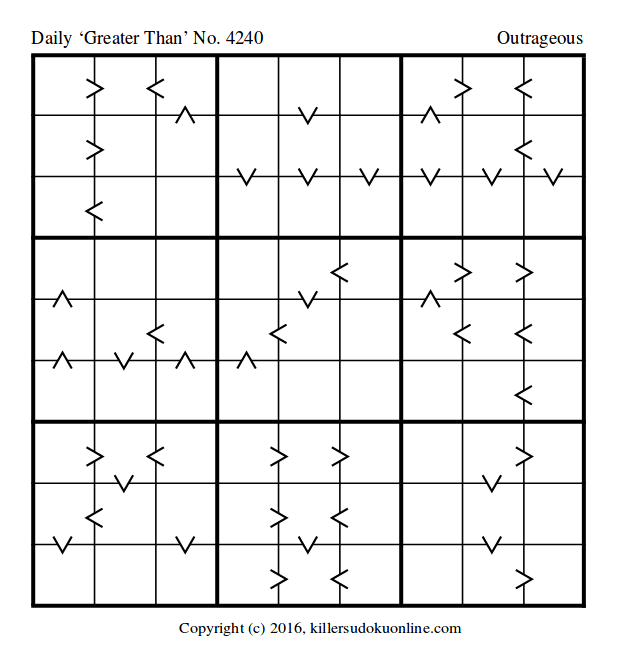
\includegraphics[scale=0.6]{puzzles/sudoku/GT/puzzle.png}
\caption{}
\end{figure}

% TODO \ref
It can be solved easily with Z3. I've took the same piece of code I used for the usual Sudoku: ().
% ( _HTML_LINK_AS_IS(`https://github.com/DennisYurichev/SAT_SMT_article/blob/master/SMT/sudoku2.py'), 

... and added this:</p>

\begin{lstlisting}
...

"""
Subsquares:

------------------------------
         |          |         
 1,1     | 1,2      | 1,3     
         |          |         
------------------------------
         |          |         
 2,1     | 2,2      | 2,3     
         |          |         
------------------------------
         |          |         
 3,1     | 3,2      | 3,3     
         |          |         
------------------------------
"""

# from http://www.killersudokuonline.com/puzzles/2017/puzzle-GD4hzi164344.pdf

# subsquare 1,1:
s.add(cells[0][0]>cells[0][1])
s.add(cells[1][0]>cells[1][1])
s.add(cells[2][0]<cells[2][1])

s.add(cells[0][1]<cells[0][2])
s.add(cells[0][2]<cells[1][2])

# subsquare 1,2:
s.add(cells[0][4]>cells[1][4])
s.add(cells[1][3]>cells[2][3])
s.add(cells[1][4]>cells[2][4])
s.add(cells[1][5]>cells[2][5])

# subsquare 1,3:
s.add(cells[0][6]>cells[0][7])
s.add(cells[0][7]<cells[0][8])
s.add(cells[0][6]<cells[1][6])
s.add(cells[1][7]<cells[1][8])
s.add(cells[1][6]>cells[2][6])
s.add(cells[1][7]>cells[2][7])
s.add(cells[1][8]>cells[2][8])

# subsquare 2,1:
s.add(cells[3][0]<cells[4][0])
s.add(cells[4][0]<cells[5][0])
s.add(cells[4][1]<cells[4][2])
s.add(cells[4][0]<cells[5][0])
s.add(cells[4][1]>cells[5][1])
s.add(cells[4][2]<cells[5][2])

# subsquare 2,2:
s.add(cells[3][4]>cells[4][4])
s.add(cells[3][4]<cells[3][5])
s.add(cells[4][3]<cells[4][4])
s.add(cells[4][3]<cells[5][3])

# subsquare 2,3:
s.add(cells[3][6]>cells[3][7])
s.add(cells[3][7]>cells[3][8])
s.add(cells[3][6]>cells[4][6])
s.add(cells[4][6]<cells[4][7])
s.add(cells[4][7]<cells[4][8])
s.add(cells[5][7]<cells[5][8])

# subsquare 3,1:
s.add(cells[6][0]>cells[6][1])
s.add(cells[6][1]<cells[6][2])
s.add(cells[6][1]>cells[7][1])
s.add(cells[7][0]<cells[7][1])
s.add(cells[7][0]>cells[8][0])
s.add(cells[7][2]>cells[8][2])

# subsquare 3,2:
s.add(cells[6][3]>cells[6][4])
s.add(cells[6][4]>cells[6][5])
s.add(cells[7][3]>cells[7][4])
s.add(cells[7][4]<cells[7][5])
s.add(cells[8][3]>cells[8][4])
s.add(cells[8][4]<cells[8][5])
s.add(cells[7][4]>cells[8][4])

# subsquare 3,3:
s.add(cells[6][7]>cells[6][8])
s.add(cells[6][7]>cells[7][7])
s.add(cells[7][7]>cells[8][7])
s.add(cells[8][7]>cells[8][8])

...
\end{lstlisting}

( The full file: \url{https://github.com/DennisYurichev/yurichev.com/.../sudoku_GT.py} )

The puzzle marked as ``Outrageous'' (for humans?), however it took $\approx 30$ seconds
on my old Intel Xeon E3-1220 3.10GHz to solve it:

\begin{lstlisting}
7 3 4 6 9 2 5 1 8
2 1 5 8 3 7 9 4 6
6 8 9 5 1 4 7 2 3
1 7 3 2 8 9 6 5 4
5 4 6 1 7 3 2 8 9
9 2 8 4 5 6 1 3 7
8 6 7 3 2 1 4 9 5
4 5 2 9 6 8 3 7 1
3 9 1 7 4 5 8 6 2
\end{lstlisting}


\subsubsection{Solving Killer Sudoku}

I've found this on \url{https://krazydad.com/killersudoku/sfiles/KD_Killer_ST16_8_v52.pdf}:

\begin{figure}[H]
\centering
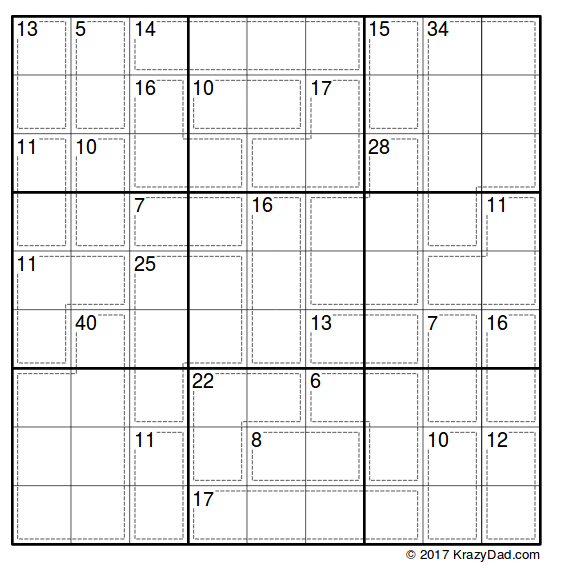
\includegraphics[scale=0.6]{puzzles/sudoku/killer/puzzle.png}
\caption{}
\end{figure}

There are ``cages'', each cage must have distinct digits,
and its sum must be equal to the number written there in a manner of crossword.
See also: \url{https://en.wikipedia.org/wiki/Killer_sudoku}.

This is also piece of cake for Z3.
% TODO \ref
I've took the same piece of code I used for usual Sudoku ( \url{...sudoku2.py} ).

\begin{lstlisting}
...

cage=[cells[0][0], cells[1][0]]
s.add(Distinct(*cage))
s.add(Sum(*cage)==13)

cage=[cells[0][1], cells[1][1]]
s.add(Distinct(*cage))
s.add(Sum(*cage)==5)

cage=[cells[0][2], cells[0][3], cells[0][4], cells[0][5]]
s.add(Distinct(*cage))
s.add(Sum(*cage)==14)

cage=[cells[0][6], cells[1][6]]
s.add(Distinct(*cage))
s.add(Sum(*cage)==15)

cage=[cells[0][7], cells[0][8], cells[1][7], cells[1][8], cells[2][7], cells[2][8], cells[3][7]]
s.add(Distinct(*cage))
s.add(Sum(*cage)==34)

cage=[cells[1][2], cells[2][2], cells[2][3]]
s.add(Distinct(*cage))
s.add(Sum(*cage)==16)

cage=[cells[1][3], cells[1][4]]
s.add(Distinct(*cage))
s.add(Sum(*cage)==10)

cage=[cells[1][5], cells[2][4], cells[2][5]]
s.add(Distinct(*cage))
s.add(Sum(*cage)==17)

cage=[cells[2][6], cells[3][5], cells[3][6], cells[4][5], cells[4][6]]
s.add(Distinct(*cage))
s.add(Sum(*cage)==28)

cage=[cells[3][2], cells[3][3]]
s.add(Distinct(*cage))
s.add(Sum(*cage)==7)

cage=[cells[3][4], cells[4][4], cells[5][4]]
s.add(Distinct(*cage))
s.add(Sum(*cage)==16)

cage=[cells[3][8], cells[4][7], cells[4][8]]
s.add(Distinct(*cage))
s.add(Sum(*cage)==11)

cage=[cells[4][0], cells[4][1], cells[5][0]]
s.add(Distinct(*cage))
s.add(Sum(*cage)==11)

cage=[cells[4][2], cells[4][3], cells[5][2], cells[5][3], cells[6][2]]
s.add(Distinct(*cage))
s.add(Sum(*cage)==25)

cage=[cells[5][1], cells[6][0], cells[6][1], cells[7][0], cells[7][1], cells[8][0], cells[8][1]]
s.add(Distinct(*cage))
s.add(Sum(*cage)==40)

cage=[cells[5][5], cells[5][6]]
s.add(Distinct(*cage))
s.add(Sum(*cage)==13)

cage=[cells[5][7], cells[6][7]]
s.add(Distinct(*cage))
s.add(Sum(*cage)==7)

cage=[cells[5][8], cells[6][8]]
s.add(Distinct(*cage))
s.add(Sum(*cage)==16)

cage=[cells[6][3], cells[6][4], cells[7][3]]
s.add(Distinct(*cage))
s.add(Sum(*cage)==22)

cage=[cells[6][5], cells[6][6], cells[7][6]]
s.add(Distinct(*cage))
s.add(Sum(*cage)==6)

cage=[cells[7][2], cells[8][2]]
s.add(Distinct(*cage))
s.add(Sum(*cage)==11)

cage=[cells[7][4], cells[7][5]]
s.add(Distinct(*cage))
s.add(Sum(*cage)==8)

cage=[cells[7][7], cells[8][7]]
s.add(Distinct(*cage))
s.add(Sum(*cage)==10)

cage=[cells[7][8], cells[8][8]]
s.add(Distinct(*cage))
s.add(Sum(*cage)==12)

cage=[cells[8][3], cells[8][4], cells[8][5], cells[8][6]]
s.add(Distinct(*cage))
s.add(Sum(*cage)==17)

...
\end{lstlisting}

( The full file: \url{...killer_sudoku.py} )

The puzzle marked as ``Super-Tough Killer Sudoku Puzzle'' (again, for humans?),
however it took $\approx 30$ seconds on my old Intel Xeon E3-1220 3.10GHz to solve it:

\begin{lstlisting}
5 3 4 7 1 2 8 9 6
8 2 1 4 6 9 7 5 3
9 6 7 8 3 5 4 2 1
2 4 6 1 9 7 3 8 5
7 1 9 3 5 8 6 4 2
3 8 5 6 2 4 9 1 7
4 7 2 5 8 3 1 6 9
6 5 8 9 7 1 2 3 4
1 9 3 2 4 6 5 7 8
\end{lstlisting}


\subsubsection{KLEE}

I've also rewritten Sudoku example (\ref{sudoku_SMT}) for KLEE:

\lstinputlisting[numbers=left]{puzzles/sudoku/KLEE/klee_sudoku_or1.c}

Let's run it:

\begin{lstlisting}
% clang -emit-llvm -c -g klee_sudoku_or1.c
...

\$ time klee klee_sudoku_or1.bc
KLEE: output directory is "/home/klee/klee-out-98"
KLEE: WARNING: undefined reference to function: klee_assert
KLEE: WARNING ONCE: calling external: klee_assert(0)
KLEE: ERROR: /home/klee/klee_sudoku_or1.c:93: failed external call: klee_assert
KLEE: NOTE: now ignoring this error at this location

KLEE: done: total instructions = 7512
KLEE: done: completed paths = 161
KLEE: done: generated tests = 161

real    3m44.111s
user    3m43.319s
sys     0m0.951s
\end{lstlisting}

Now this is really slower (on my Intel Core i3-3110M 2.4GHz notebook) in comparison to Z3Py solution (\ref{sudoku_SMT}).

But the answer is correct:

\begin{lstlisting}
% ls klee-last | grep err
test000161.external.err

% ktest-tool --write-ints klee-last/test000161.ktest
ktest file : 'klee-last/test000161.ktest'
args       : ['klee_sudoku_or1.bc']
num objects: 1
object    0: name: b'cells'
object    0: size: 81
object    0: data: b'\x01\x04\x05\x03\x02\x07\x06\t\x08\x08\x03\t\x06\x05\x04\x01\x02\x07\x06\x07\x02\t\x01\x08\x05\x04\x03\x04\t\x06\x01\x08\x05\x03\x07\x02\x02\x01\x08\x04\x07\x03\t\x05\x06\x07\x05\x03\x02\t\x06\x04\x08\x01\x03\x06\x07\x05\x04\x02\x08\x01\t\t\x08\x04\x07\x06\x01\x02\x03\x05\x05\x02\x01\x08\x03\t\x07\x06\x04'
\end{lstlisting}

Character \TT{\textbackslash{}t} has code of 9 in C/C++,
and KLEE prints byte array as a C/C++ string, so it shows some values in such way.
We can just keep in mind that there is 9 at the each place where we see \TT{\textbackslash{}t}.
The solution, while not properly formatted, correct indeed.

By the way, at lines 42 and 43 you may see how we tell to KLEE that all array elements must be within some limits.
If we comment these lines out, we've got this:

\begin{lstlisting}
% time klee klee_sudoku_or1.bc
KLEE: output directory is "/home/klee/klee-out-100"
KLEE: WARNING: undefined reference to function: klee_assert
KLEE: ERROR: /home/klee/klee_sudoku_or1.c:51: overshift error
KLEE: NOTE: now ignoring this error at this location
KLEE: ERROR: /home/klee/klee_sudoku_or1.c:51: overshift error
KLEE: NOTE: now ignoring this error at this location
KLEE: ERROR: /home/klee/klee_sudoku_or1.c:51: overshift error
KLEE: NOTE: now ignoring this error at this location
...
\end{lstlisting}

KLEE warns us that shift value at line 51 is too big.
Indeed, KLEE may try all byte values up to 255 (0xFF), which are pointless to use there,
and may be a symptom of error or bug, so KLEE warns about it. % FIXME chk spelling

Now let's use \TT{klee\_assume()} again:

\lstinputlisting{puzzles/sudoku/KLEE/klee_sudoku_or2.c}

\begin{lstlisting}
% time klee klee_sudoku_or2.bc
KLEE: output directory is "/home/klee/klee-out-99"
KLEE: WARNING: undefined reference to function: klee_assert
KLEE: WARNING ONCE: calling external: klee_assert(0)
KLEE: ERROR: /home/klee/klee_sudoku_or2.c:93: failed external call: klee_assert
KLEE: NOTE: now ignoring this error at this location

KLEE: done: total instructions = 7119
KLEE: done: completed paths = 1
KLEE: done: generated tests = 1

real    0m35.312s
user    0m34.945s
sys     0m0.318s
\end{lstlisting}

That works much faster: perhaps KLEE indeed handle this \textit{intrinsic} in a special way.
And, as we see, the only one path has been found (one we actually interesting in it) instead of 161.

It's still much slower than Z3Py solution, though.


\subsubsection{Sudoku in SAT}
\label{Sudoku_SAT}

One might think that we can encode each 1..9 number in binary form: 5 bits or variables would be enough.
But there is even simpler way: allocate 9 bits, where only one bit will be \textit{True}.
The number 1 can be encoded as [1, 0, 0, 0, 0, 0, 0, 0, 0], the number 3 as [0, 0, 1, 0, 0, 0, 0, 0, 0], etc.
Seems uneconomical? Yes, but other operations would be simpler.

First of all, we'll reuse important \TT{POPCNT1} function I've described earlier: \ref{POPCNTOne}.

The second important operation we need to invent is making 9 numbers unique.
If each number is encoded as 9-bits vector, 9 numbers can form a matrix, like:

\begin{lstlisting}
0 0 0 0 0 0 1 0 0 <- 1st number
0 0 0 0 0 1 0 0 0 <- 2nd number
0 1 0 0 0 0 0 0 0 <- ...
0 0 1 0 0 0 0 0 0 <- ...
0 0 0 0 0 0 0 0 1 <- ...
0 0 0 0 1 0 0 0 0 <- ...
0 0 0 0 0 0 0 1 0 <- ...
1 0 0 0 0 0 0 0 0 <- ...
0 0 0 1 0 0 0 0 0 <- 9th number
\end{lstlisting}

Now we will use a \TT{POPCNT1} function to make each row in the matrix to contain only one \textit{True} bit, that will
preserve consistency in encoding, since no vector can contain more than 1 \textit{True} bit, or no \textit{True} bits at all.
Then we will use a \TT{POPCNT1} function again to make all columns in the matrix to have only one single \textit{True} bit.
That will make all rows in matrix unique, in other words, all 9 encoded numbers will always be unique.

After applying \TT{POPCNT1} function 9+9=18 times we'll have 9 unique numbers in 1..9 range.

Using that operation we can make each row of Sudoku puzzle unique, each column unique and also each $3 \cdot 3=9$ box.

\lstinputlisting[style=custompy]{puzzles/sudoku/SAT/sudoku_SAT.py}
( \url{https://github.com/DennisYurichev/SAT_SMT_by_example/blob/master/puzzles/sudoku/SAT/sudoku_SAT.py} )

The \TT{make\_distinct\_bits\_in\_vector()} function preserves consistency of encoding.\\
The \TT{make\_distinct\_vectors()} function makes 9 numbers unique.\\
The \TT{cvt\_vector\_to\_number()} decodes vector to number.\\
The \TT{number\_to\_vector()} encodes number to vector.\\
The \TT{main()} function has all necessary calls to make rows/columns/$3\cdot 3$ boxes unique.

That works:

\begin{lstlisting}
% python sudoku_SAT.py
len(clauses)= 12195
1 4 5 3 2 7 6 9 8
8 3 9 6 5 4 1 2 7
6 7 2 9 1 8 5 4 3
4 9 6 1 8 5 3 7 2
2 1 8 4 7 3 9 5 6
7 5 3 2 9 6 4 8 1
3 6 7 5 4 2 8 1 9
9 8 4 7 6 1 2 3 5
5 2 1 8 3 9 7 6 4
\end{lstlisting}

Same solution as earlier: \ref{sudoku_SMT}.

Picosat tells this SAT instance has only one solution.
Indeed, as they say, true Sudoku puzzle can have only one solution.

\paragraph{Getting rid of one POPCNT1 function call}
\label{OR_in_POPCNT1}

To make 9 unique 1..9 numbers we can use \TT{POPCNT1} function to make each row in matrix be unique and
use \textit{OR} boolean operation for all columns.
That will have merely the same effect: all rows has to be unique to make each column to be evaluated
to \textit{True} if all variables in column are OR'ed.
(I will do this in the next example: \ref{Zebra_SAT}.)

That will make 3447 clauses instead of 12195, but somehow, SAT solvers works slower. No idea why.



